\documentclass[10pt,twocolumn,letterpaper]{article}

\usepackage{iccv}
\usepackage{times}
\usepackage{epsfig}
\usepackage{graphicx}
\usepackage{amsmath}
\usepackage{amssymb}

\usepackage{pbox}
\usepackage{verbatim}
\usepackage{bm}
\usepackage{microtype}
\usepackage{url}
\usepackage{multirow}
\usepackage{tikz}
\usetikzlibrary{shadows,trees}

\newlength{\eqs}
\setlength{\eqs}{-0.04in}

\usepackage{enumitem}
\setitemize[0]{leftmargin=15pt}

\newenvironment{tight_itemize}{
\begin{itemize}[leftmargin=10pt]
  \setlength{\topsep}{0pt}
  \setlength{\itemsep}{0pt}
  \setlength{\parskip}{0pt}
  \setlength{\parsep}{0pt}
}{\end{itemize}}


% Include other packages here, before hyperref.

% If you comment hyperref and then uncomment it, you should delete
% egpaper.aux before re-running latex.  (Or just hit 'q' on the first latex
% run, let it finish, and you should be clear).
\usepackage[pagebackref=true,breaklinks=true,letterpaper=true,colorlinks,bookmarks=false]{hyperref}

\iccvfinalcopy % *** Uncomment this line for the final submission

%\newcommand{\bm}{\mathbf{}}
% New math commands/abreviations

\newcommand{\bA}{\mathbf{A}}
\newcommand{\bB}{\mathbf{B}}
\newcommand{\bC}{\mathbf{C}}
\newcommand{\bD}{\mathbf{D}}
\newcommand{\bE}{\mathbf{E}}
\newcommand{\bF}{\mathbf{F}}
\newcommand{\bG}{\mathbf{G}}
\newcommand{\bH}{\mathbf{H}}
\newcommand{\bI}{\mathbf{I}}
\newcommand{\bJ}{\mathbf{J}}
\newcommand{\bK}{\mathbf{K}}
\newcommand{\bL}{\mathbf{L}}
\newcommand{\bM}{\mathbf{M}}
\newcommand{\bN}{\mathbf{N}}
\newcommand{\bO}{\mathbf{O}}
\newcommand{\bP}{\mathbf{P}}
\newcommand{\bQ}{\mathbf{Q}}
\newcommand{\bR}{\mathbf{R}}
\newcommand{\bS}{\mathbf{S}}
\newcommand{\bT}{\mathbf{T}}
\newcommand{\bU}{\mathbf{U}}
\newcommand{\bV}{\mathbf{V}}
\newcommand{\bW}{\mathbf{W}}
\newcommand{\bX}{\mathbf{X}}
\newcommand{\bY}{\mathbf{Y}}
\newcommand{\bZ}{\mathbf{Z}}

\newcommand{\ba}{\mathbf{a}}
%\newcommand{\bb}{\mathbf{b}}
\newcommand{\bc}{\mathbf{c}}
\newcommand{\bd}{\mathbf{d}}
\newcommand{\be}{\mathbf{e}}
%\newcommand{\bf}{\mathbf{f}}
\newcommand{\bg}{\mathbf{g}}
\newcommand{\bh}{\mathbf{h}}
\newcommand{\bi}{\mathbf{i}}
\newcommand{\bj}{\mathbf{j}}
\newcommand{\bk}{\mathbf{k}}
\newcommand{\bl}{\mathbf{l}}
%\newcommand{\bm}{\mathbf{m}}
\newcommand{\bn}{\mathbf{n}}
%\newcommand{\bo}{\mathbf{o}}
\newcommand{\bp}{\mathbf{p}}
\newcommand{\bq}{\mathbf{q}}
\newcommand{\br}{\mathbf{r}}
\newcommand{\bs}{\mathbf{s}}
\newcommand{\bt}{\mathbf{t}}
\newcommand{\bu}{\mathbf{u}}
\newcommand{\bv}{\mathbf{v}}
\newcommand{\bw}{\mathbf{w}}
\newcommand{\bx}{\mathbf{x}}
\newcommand{\by}{\mathbf{y}}
\newcommand{\bz}{\mathbf{z}}

\newcommand{\bff}{\mathbf{f}}

\newcommand{\bo}{\mathbf{0}}
\newcommand{\tx}{\tilde{\mathbf{x}}}


\newcommand{\hbn}{{\widehat{\mathbf{n}}}}
\newcommand{\hbs}{{\widehat{\mathbf{s}}}}
\newcommand{\hbh}{{\widehat{\mathbf{h}}}}
\newcommand{\hbv}{{\widehat{\mathbf{v}}}}
\newcommand{\hbw}{{\widehat{\mathbf{w}}}}
\newcommand{\hbc}{{\widehat{\mathbf{c}}}}

\newcommand{\hh}{{\widehat{h}}}
\newcommand{\hn}{{\widehat{n}}}
\newcommand{\hx}{{\widehat{x}}}
\newcommand{\hy}{{\widehat{y}}}
\newcommand{\hz}{{\widehat{z}}}


% Mathcal definitions
\newcommand{\cS}{\mathcal{S}}
\newcommand{\cD}{\mathcal{D}}
\newcommand{\cP}{{\mathcal{P}}}
\newcommand{\cU}{{\mathcal{U}}}
\newcommand{\cV}{{\mathcal{V}}}
\newcommand{\cE}{{\mathcal{E}}}
\newcommand{\cQ}{{\mathcal{Q}}}
\newcommand{\cG}{{\mathcal{G}}}
\newcommand{\cB}{{\mathcal{B}}}
\newcommand{\cI}{\mathcal{I}}
\newcommand{\cL}{\mathcal{L}}
\newcommand{\cR}{{\mathcal{R}}}
\newcommand{\cC}{{\mathcal{C}}}
\newcommand{\cO}{{\mathcal{O}}}
\newcommand{\cX}{{\mathcal{X}}}



% Mathbb definitions
\newcommand{\bbp}{\mathbb{P}}
\newcommand{\bbP}{\mathbb{P}}
\newcommand{\bbQ}{\mathbb{Q}}
\newcommand{\bbr}{\mathbb{R}}
\newcommand{\bbR}{\mathbb{R}}
\newcommand{\bbS}{\mathbb{S}}
\newcommand{\bbN}{\mathbb{N}}



% Mathbm definitions
\newcommand{\balpha}{{\bm{\alpha}}}
\newcommand{\bbeta}{{\bm{\beta}}}
\newcommand{\bgamma}{{\bm{\gamma}}}
\newcommand{\bepsilon}{{\bm{\epsilon}}}
\newcommand{\bmu}{{\bm{\mu}}}
\newcommand{\bpi}{\bm{\pi}}
\newcommand{\brho}{\bm{\rho}}
\newcommand{\bomega}{\bm{\omega}}
\newcommand{\bOmega}{\bm{\Omega}}
\newcommand{\bSigma}{\bm{\Sigma}}
\newcommand{\bGamma}{\bm{\Gamma}}



\newcommand{\id}{\mathbf{I}}
\newcommand{\tid}{\tilde{\id}}
\newcommand{\st}{{\textrm{subject to }}}


\newcommand{\bpm}{{\widehat{\bP}}}
\newcommand{\bxm}{{\widehat{\mathbf{X}}}}
\newcommand{\winf}{{{\bm{\Omega}}_\infty}}
%\newcommand{\bw}{{{\bm{\omega}}^*}}
\newcommand{\bwi}{{{\bm{\omega}}_i^*}}
\newcommand{\bwone}{{{\bm{\omega}}_1^*}}
\newcommand{\diac}{{{\bm{\omega}}^*}}
\newcommand{\iac}{{{\bm{\omega}}}}
\newcommand{\ac}{{{\bm{\Omega}}_\infty}}
\newcommand{\diaci}{{{\bm{\omega}}_i^*}}
\newcommand{\diacone}{{{\bm{\omega}}_1^*}}
\newcommand{\w}{{{\bm{\omega}}^*}}
\newcommand{\daq}{{\mathbf{Q}}_\infty^*}
\newcommand{\adq}{{\mathbf{Q}}_\infty^*}
\newcommand{\pinf}{{\bm{\pi}}_\infty}
\newcommand{\hinf}{{{\bH}_\infty}}
\newcommand{\hinft}{{{\bH}^\top_\infty}}
\newcommand{\hinfi}{{{\bH}^i_\infty}}
\newcommand{\hinfit}{{{\bH}^{i\top}_\infty}}
\newcommand{\hinfj}{{{\bH}^j_\infty}}
\newcommand{\hinfjt}{{{\bH}^{j\top}_\infty}}
\newcommand{\intval}[2]{[\, #1, #2 \, ]}
\newcommand{\camo}{\left[ \: \id \: \vert \: \bo \: \right]}
\newcommand{\cama}{\left[ \: \bA \: \vert \: \ba \: \right]}
\newcommand{\camr}{\left[ \: \bR \: \vert \: \bt \: \right]}
\newcommand{\camai}{\left[ \: \bA_i \: \vert \: \ba_i \: \right]}
\newcommand{\camri}{\left[ \: \bR_i \: \vert \: \bt_i \: \right]}

%\newcommand{\algorithmiccomment}[1]{//#1}
\newcommand{\lb}{\operatorname{\bf{Bound}}}
\newcommand{\branch}{\operatorname{\bf{Branch}}}
\newcommand{\feasible}{\operatorname{\bf{Feasible}}}
\newcommand{\trace}{\operatorname{Tr}}
\newcommand{\convenv}{\operatorname{\bf{convenv}}}
\newcommand{\rectangle}{Q}

\newcommand{\epi}{\operatorname{\bf{epi}}}
\newcommand{\dom}{\operatorname{\bf{dom}}}

\newcommand{\ophi}{f}
\newcommand{\phimin}{\ophi_{\text{min}}}
\newcommand{\philb}{\ophi_{\text{lb}}}
\newcommand{\phiub}{\ophi_{\text{ub}}}

\newcommand{\cvx}{{\mathrm{convex\_env}}}
\newcommand{\ccv}{{\mathrm{concave\_env}}}

\newcommand{\conc}[1]{\operatorname{conc}{#1}}
\newcommand{\conv}[1]{\operatorname{conv}{#1}}

%\newcommand{\deg}[1]{\operatorname{deg}{#1}}

\newcommand{\lmi}[1]{\operatorname{LMI}{#1}}

\newcommand{\fa}{\alpha}
\newcommand{\fb}{\beta}
\newcommand{\fc}{\gamma}


%\newcommand{\tr}{^\top}

\newcommand{\xlt}{x_l^{1/3}}
\newcommand{\xut}{x_u^{1/3}}
\newcommand{\tlt}{t_l^{1/3}}
\newcommand{\tut}{t_u^{1/3}}
\newcommand{\xl}{x_l}
\newcommand{\xu}{x_u}
\newcommand{\yl}{y_l}
\newcommand{\yu}{y_u}
\newcommand{\tl}{t_l}
\newcommand{\tu}{t_u}
\newcommand{\yp}{y_p}
\newcommand{\ypd}{y'_p}
\newcommand{\tp}{t_p}
\newcommand{\fl}{\frac{x - \xl}{\xu - \xl}}
\newcommand{\fu}{\frac{\xu - x}{\xu - \xl}}


% Bilinear definitions
\newcommand{\cl}{{\psi}^l}
\newcommand{\cu}{{\psi}^u}
\newcommand{\rect}{Q}
\newcommand{\cond}[1]{\operatorname{{\mathcal{C}}}{#1}}
\newcommand{\vol}[1]{\operatorname{vol}{#1}}

%\newcommand{\phimin}[1]{\operatorname{\Phi_{\textrm{min}}}{#1}}
%\newcommand{\philb}[1]{\operatorname{\Phi_{\textrm{lb}}}{#1}}
%\newcommand{\phiub}[1]{\operatorname{\Phi_{\textrm{ub}}}{#1}}


%\newcommand{\rank}{{\mathbf{rank}}}
%\newcommand{\diag}{{\mathrm{diag}}}

\newcommand{\rank}[1]{\operatorname{rank}{#1}}

%\newcommand{\bx}{x} %general unknown x
%\newcommand{\bX}{X} %scene point

\newcommand{\ix}{\bx} %image point
\newcommand{\ixa}{u} %1st coordinate of image point
\newcommand{\ixb}{v} %2nd coordinate of image point
\newcommand{\bXa}{U} %1st coordinate of scene point
\newcommand{\bXb}{V} %2nd coordinate of scene point
\newcommand{\bXc}{W} %3rd coordinate of scene point

\newcommand{\tr}{^\top}

\newcommand{\Linf}{L_{\infty}}
\newcommand{\Ltwo}{L_{2}}
\newcommand{\Lone}{L_{1}}
\newcommand{\Lp}{L_{p}}
\newcommand{\Lq}{L_{q}}

\def\smallmat#1{\left[\begin{smallmatrix}#1\end{smallmatrix}\right]}



\newcommand{\brs}{\bR_0}
\newcommand{\bts}{\bt_0}
\newcommand{\bzero}{\mathbf{0}}
\newcommand{\bdx}{\mathbf{dx}}

\newcommand{\p}{\partial}


\newcommand{\del}[1]{\nabla_{#1}}
\newcommand{\I}{\mathbf{I}}
\newcommand{\II}{\mathbf{II}}
\newcommand{\skewsymm}[1]{[{#1}]_\times}





% 3D pose of the cars and ego motion
\newcommand{\pos}[2]{\mathbf{p}^{#1}({#2})}
\newcommand{\ori}[2]{\mathbf{\omega}^{#1}(#2)}
\newcommand{\state}[2]{\mathbf{s}^{#1}(#2)}

% ego pose
\newcommand{\egop}[1][t]{\pos{c}{#1}}
\newcommand{\egoo}[1][t]{\ori{c}{#1}}
\newcommand{\egos}[1][t]{\state{c}{#1}}

% relative pose between camera and car $i$
\newcommand{\relp}[2]{\Omega^{#1}(#2)}
\newcommand{\relpz}[2]{\Omega_z^{#1}(#2)}

% 3D tracks on car $i$ in its own coordinate frame
\newcommand{\tracklets}{\mathbf{X}^{i}_o}
\newcommand{\tracklet}[1]{\mathbf{x}^{i}_{#1}}
% track projections on camera
\newcommand{\trackpit}[2]{\mathbf{u}_{#1}(#2)}
\newcommand{\trackp}[1]{\mathbf{u}_j(#1)}
\newcommand{\trackpj}[1]{\mathbf{u}_j(#1)}
% Unclassified track point projected on camera
\newcommand{\ucTrackp}{\mathbf{u}(t)}


% dimensions of car $i$
\newcommand{\dimsn}[1]{\mathbf{B}^{#1}}
\newcommand{\expDimsn}{\hat{\mathbf{B}}}

% projection function
\newcommand{\projectionOf}[1]{\pi_{\relp{i}{t}}\left(#1\right)}
\newcommand{\projectionOft}[1]{\pi_{\relp{i}{t+1}}\left(#1\right)}
\newcommand{\centerProj}{\bar{\pi}_{\relp{i}{t}}(\dimsn{i})}
\newcommand{\cornerProj}[1]{\pi^{#1}_{\relp{i}{t}}(\dimsn{i})}
\newcommand{\triangleProj}[1]{\triangle^{#1}_{\relp{i}{t}}(\dimsn{i})}

% bounding box corners on image
\newcommand{\bbt}[2]{\mathbf{d}^{#1}({#2})}
\newcommand{\bb}[1]{\mathbf{d}^{#1}(t)}


\newcommand{\Energy}[1]{\mathcal{E}^{it}_{\text{#1}}}
\newcommand{\pEnergy}[1]{\mathcal{E}^{ijt}_{\text{#1}}}
% Weighted energy
\newcommand{\WEnergy}[1]{\lambda_{\text{#1}}\Energy{#1}}
\newcommand{\WpEnergy}[1]{\lambda_{\text{#1}}\pEnergy{#1}}
\newcommand{\EnergyCol}{\mathcal{E}^{ijt}_{\text{col}}}
\newcommand{\WEnergyCol}{\lambda_{\text{col}}\EnergyCol}

\newcommand{\EnergyBBoxNoOcc}{\Energy{detectNoOcc}}
\newcommand{\EnergyBBox}{\Energy{detect}}
\newcommand{\EnergyTrack}{ \pEnergy{track}}
\newcommand{\EnergyTrackNoOcc}{\pEnergy{trackNoOcc}}
\newcommand{\EnergyLane}{\Energy{lane}}
\newcommand{\EnergySize}{\Energy{size}}
\newcommand{\EnergyDyn}{\Energy{dyn}}
\newcommand{\EnergyDynHol}{\Energy{dyn-hol}}
\newcommand{\EnergyDynOri}{\Energy{dyn-ori}}
\newcommand{\EnergyDynVel}{\Energy{dyn-vel}}

\newcommand{\occFreeProj}[1]{\Pi_{\relp{i}{t}}(#1)}
\newcommand{\minx}{x_{\text{min}}}
\newcommand{\miny}{y_{\text{min}}}
\newcommand{\maxx}{x_{\text{max}}}
\newcommand{\maxy}{y_{\text{max}}}
\newcommand{\frontface}{F^i_\text{FF}(t)}

\newcommand{\occ}[1]{o({#1})}
\newcommand{\face}{F^i_k(t)}

\newcommand{\invProjectionOf}[1]{\pi^{-1}_{\relp{i}{t}}\left(#1\right)}
\newcommand{\invProjectionOftm}[1]{\pi^{-1}_{\relp{i}{t-1}}\left(#1\right)}
\newcommand{\occf}{f^i_{occ}(\mathbf{x}_j)}
\newcommand{\occftot}{f_{occ}(\mathbf{x}_j)}
\newcommand{\occft}[1]{f_{occ}(#1)}

\newcommand{\ray}{\hat{\mathbf{r}}_j}
\newcommand{\occfray}{f_{occ}(\lambda\ray)}
\newcommand{\lambdadist}{f_{\lambda}(\trackpj{t-1}, \lambda)}

\newcommand{\occfxi}{L(\mathbf{x}; \pos{i}{t-1}, \Sigma_i)}
\newcommand{\occfi}{L(\lambda \ray; \pos{i}{t-1}, \Sigma_i)}
\newcommand{\assocP}{a^{ij}(\lambda)}
\newcommand{\assocPk}{a^{ij}(\lambda_k)}

\newcommand{\Ereproj}{E^{ij}_{\text{reproj}}}
\newcommand{\Ptransarg}[1]{P^{j}_{\text{transmission}}(#1)}
\newcommand{\Ptrans}{\Ptransarg{\lambda}}
\newcommand{\Ptransmud}{P^{j}_{\text{transmission}}(\mu^{i}_d)}
\newcommand{\Prefl}{P^{ij}_{\text{reflection}}(\lambda)}
\newcommand{\dishort}{d_i(\mathbf{x})}

\newcommand{\Lu}{L_u(\mathbf{u}, \mu^i_u,\Sigma^i_u)}
\newcommand{\Llambda}{L_{\lambda}(\mathbf{u}, \lambda; \mu^i_d)}

\newcommand{\Gauss}{\mathcal{N}}
\newcommand{\PropDist}{\mathcal{W}_j}

\newcommand{\muijl}{\mu^{ij}_{\lambda}}
\newcommand{\sigmaijl}{\sigma^{ij}_{\lambda}}

\newcommand{\Sigmait}{\bSigma^{i^{-1}}_o}

\newcommand{\muit}{\bmu^{i}_o}
\newcommand{\Sigmaic}{\bSigma'^{i^{-1}}_c}

\newcommand{\muic}{{\bmu^{i}_c}}
\newcommand{\Sigmaicf}{\bSigma^{i^{-1}}_c}
\newcommand{\Sigmaicfinv}{\Sigma^{i}_c}

\newcommand{\muiu}{\mu^{i}_t}
\newcommand{\Sigmaiu}{\Sigma^{i^{-1}}_u}

\newcommand{\uv}[1]{\hat{\mathbf{#1}}}
\newcommand{\Tr}[3]{{}^{#1}{#2}_{#3}}
\newcommand{\xymin}[1]{#1_{\text{min}}}
\newcommand{\xymax}[1]{#1_{\text{max}}}
\newcommand{\vect}[1]{\mathbf{#1}}
\newcommand{\map}{\vect{x}}

\newcommand{\xt}{\mathbf{x}_t}
\newcommand{\xc}{\mathbf{x}_c}

\newcommand{\Rctot}{\bR}
\newcommand{\tctot}{\bt}

\newcommand{\tcmut}{\bt'}


\newcommand{\Beizer}{B\'eizer }

\newcommand{\LaneUncertainty}[1]{\Sigma_{L_m}(#1)}
\newcommand{\projOnLane}[1]{\pi_{L_m(k)}(#1)}
\newcommand{\meandepth}[1]{\nu_#1}


%\DeclareMathSymbol{\Tangent}
\DeclareMathOperator{\diag}{diag}
\DeclareMathOperator{\sech}{sech}
\DeclareMathOperator{\poly}{poly}
%\DeclareMathOperator*{\argmin}{\arg\min}



\DeclareMathOperator*{\argmin}{\arg\min}

\def\iccvPaperID{639} % *** Enter the ICCV Paper ID here
\def\httilde{\mbox{\tt\raisebox{-.5ex}{\symbol{126}}}}

% Pages are numbered in submission mode, and unnumbered in camera-ready
\ificcvfinal\pagestyle{empty}\fi
\begin{document}

%%%%%%%%% TITLE
\title{Continous occlusion models and traffic scene understanding}
\author{Vikas Dhiman\\
  University of Michigan\\
  Ann Arbor, MI, USA\\
  {\tt\small dhiman@umich.edu}
  \and
  Manmohan Chandrakar\\
  NEC Laboratories America Ltd\\
  Cupertino, CA, USA\\
  {\tt\small manu@nec-labs.com}
  \and
  Jason J Corso\\
  University of Michigan\\
  Ann Arbor, MI, USA\\
  {\tt\small jjcorso@umich.edu}
}
\maketitle
%%%%%%%%% ABSTRACT
\begin{abstract}
  %Problem:
  3D localization in road scenes from monocular video is an important problem
  for applications in autonomous driving. We propose a probabilistic graphical
  model based framework to estimate 3D localization of traffic participants in
  road scenes.  We use object detections, point tracks, egomotion, estimated
  ground truth, GPS and map information as an input to our system.
  Given this input we compute 6DOF 3D localization of traffic participants
  along with their dimensions (height, width and length).
  We also introduce a novel perspective to the soft occlusion models where a
  region in space is viewed in terms of reflection and transmission
  probability.
  We test and train our model on KITTI dataset and show that our occlusion
  model works better than the baseline method of bounding boxes. We also show
  that our 3D localization results with monocular video input are comparable to
  (Geiger 2014) which uses stereo input.

  % Why monocular
  % Since laser scanners are expensive, we focus on solving the problem through
  % monocular video, GPS and maps as our input. Given the video we extract the 
  % Methodology
  % We formulate the problem of 3D localization in a probabilistic graphical
  % model specifically a factor graph model. We use additional heuristic
  % constraints like collision constraint, 

\end{abstract}



% \begin{tight_itemize}
%   \item Introduce the problem
%   \item Describe our approach
%   \item Contrast with Milan's work
%   \item Contrast with Andreas Geiger's work
%   \item Highlight the contributions
% \end{tight_itemize}
% \vspace{10cm}

        To accomplish fully or partial autonomous driving we need 3D
        localization of traffic participants in the scene. 
        Since laser scanners and stable wide--baseline stereo setups are
        expensive, we focus on solving the problem using monocular video, GPS
        and maps as our input. Given the video we extract detection bounding
        boxes, ground plane and point tracks.
        We formulate the problem of 3D localization in a probabilistic graphical
        model specifically a factor graph model. We use additional heuristic
        constraints like collision constraint, that leads to a global consistent solution.
        Using these multiple sources of information that provide, possibly conflicting evidence about
        the location of traffic participant, a consistent meaningful solution must be estimated. 
        We formulate the problem in factor graph
        formalism and use off-the-shelf methods for inference.

        Our main contribution is a novel continous occlusion aware 3D object
        modeling. This modeling is more principled than the continuous occlusion models proposed by Milan et al~\cite{Milan_etal_2014}, as our model is in 3D and derives it reasoning from fundamentals of optics. 
         In other words, we provide a optics based
        perspective to occlusion modeling. Also we propose a unique point
        tracks energy that is based on reprojection error and occlusion based
        association probability. Our experiments show that association
        probability provides more accurate point to object association than
        using simple bounding box based methods.



% % This work is a triple dip: 
% (1) PGM course (2) Qualifier project (3) ICCV submiission

% 
% % Message to be delivered 
% 1. To show the work done
% 2. Exemplify technical powress 
% 3. understanding of graphical models
% 4. Lessons learned: 
%   4.a) occlusion modeling doesn't help much
%   4.b) GPS/Map/Lane are useful
%   4.c) Particle Belief propagation has tough competition from fminunc


% % Course point of view (PGM)
% What is the graphical model that we used for the problem
% What inference method we used for the problem.
% How did the results match to naive realization

% What I did
% GPS/Map/lane orientatio
% Occlusion modeling
% Particle Belief propagation

% What did I learn
% GPS is much more accurate than we would like to think
% Occlusion modeling doesn't help much as we think
% PBP has a surprising competitor

% Outline
% Abstract
% 1 Introduction
% Figure explaining the pipeline?

% 1.5 Related work
\section{Related Work}
\label{sec:related}


\paragraph{Occlusion handling}
Several works in object detection consider occlusion by training a detector on visible parts of the object \cite{Gao_etal_2011,Wu_Nevatia_2007}. Occlusion reasoning based on 2D image silhouettes is used to improve detection performance in \cite{Hsiao_Herbert_2012}.  In recent years, object detectors have also considered occlusion reasoning using 3D cues, often learned from a dataset of CAD models \cite{Pepik_etal_2012,Pepik_etal_2013,Xiang_Savarese_2013}. By necessity, such frameworks are often a discrete representation of occlusion behavior, for example, in the form of a collection of occlusion masks derived from object configurations discretized over viewpoint. In constrast to these works, our occlusion modeling is also fully 3D, but allows for a continuous representation. Further, to derive 3D information, we do not use CAD models, rather we derive a probabilistic formulation based on physical insights.


Occlusion handling in tracking \cite{Kwak_etal_2012,Wu_Nevatia_2007,Milan_etal_2014}.


\paragraph{3D localization and scene understanding}
General \cite{Geiger2011, Geiger_etal_2014}.
Occlusion handling in scene understanding works \cite{Wojek_etal_2013,Zia_etal_2013,Zia_etal_2014}.


\paragraph{Motion segmentation and multibody SFM}
\cite{Tron_Vidal_2007}
\cite{Rao_etal_2010}
\cite{Brox_Malik_2010}


\cite{Schindler2006}
\cite{Ozden_etal_2010}
\cite{Namdev2012}
\cite{Kundu_etal_2011}



\paragraph{Motion segmentation}






TODO:
\vfill
\pagebreak
Related work continued
\vspace{15cm}



%
% 2 Modeling
\section{Overview of Problem and Our Approach}

\paragraph{Notation}


\begin{table}[h]
  \begin{tabular}{|l|l|}
    \hline
    Symbol & Meaning \\
    \hline
    $\pos{i}{t}$ & Position of $i$th car at time $t$\\
    $\ori{i}{t}$ & Orientation of $i$th car at time $t$\\
     $\dimsn{i}$ & 3D bounding box of the car (dimensions)\\
    $\state{i}{t}$ & State of car $=\{\pos{i}{t}, \ori{i}{t}, \dimsn{i}\}$\\
    $\egop$ & Position of camera at time $t$\\
    $\egoo$ & Orientation of camera at time $t$\\
    $\relp{i}{t}$ & Relative car pose w.r.t. camera \\
    $\tracklets$ & 3D points tracked on car $i$ in its own frame\\
    $\trackp{t}$ & Projection of $\tracklets$ in camera\\
    $\projectionOf{.}$ & Projection function for pose $\relp{i}{t}$\\
    $\bb{i}$ & 2D bounding box of the car in image\\
    \hline
  \end{tabular}
\end{table}

%%%%%%%%% BODY TEXT
\paragraph{The Model}

The objective is to find the most likely traffic participant (TP) state given
various evidences $\mathbb{E} = \{\{\trackp{t}\}, \{\bb{i}\}, \text{lane det.},
\text{map}, \text{GPS}\}$.

Mathematically, find:
\begin{align}
  \{\state{i}{t}\}^* &= \arg \max P(\{\state{i}{t}\} | \mathbb{E})
\end{align}

Bayes rule
\begin{align}
  P(\{\state{i}{t}\} | \mathbb{E}) &=
  \frac{1}{Z}P( \mathbb{E} | \{\state{i}{t}\})P(\{\state{i}{t}\})
\end{align}


Assume conditional independence according to graphical model in
\ref{fig:graphmodel}.

\begin{multline}
  P(\{\state{i}{t}\} | \mathbb{E}) =
  \frac{1}{Z}
  \prod_{t=s_i}^{e_i}\prod_{i,j: i \ne j}(P(\state{i}{t}, \state{j}{t}))\\
%
  \prod_{i=1}^{N}
  \prod_{t=s_i}^{e_i}
  P(\bb{i} | \state{i}{t})
  P(\trackp{t} | \state{i}{t})\\
  P(\state{i}{t} | L_m(t))
  P(\state{i}{t} | \state{i}{t-1})
  P(\state{i}{t})
\end{multline}

We can formulate similar objective function in negative log domain:
\footnote{TODO:Resolve inconsistency in summation absorption in energy terms.}
\begin{multline}
  -\log{P(\{\state{i}{t}\} | \mathbb{E})} = 
  Z' + \sum_{i,j:i\ne j} \sum_{t=s_i}^{e_i}  \WEnergyCol \\
  + \sum_{i=1}^N \sum_{t=s_i}^{e_i}
    \WEnergy{box}
  + \WEnergy{track}\\
  + \WEnergy{lane}
  + \WEnergy{dyn}
  + \WEnergy{prior}
\end{multline}

% Figure explaining the model within a car
% Figure explaining the model within a frame
% Figure explaining the model multiples frames
% 2.1 GPS and Lane information
% 2.2 Occlusion modeling

In this section, we introduce our representation of 3D traffic participants and our modeling of object-object occlusion relationships. We refer the reader to Figure~\ref{fig:reflectiontransimission} for an illustration of the proposed concepts.

\begin{figure}
  \usetikzlibrary{calc}
  \centering
  \begin{tikzpicture}
         \path [fill=blue!20,draw] (0,0) ellipse (1.2 and 0.7);
     \path [fill=green!20,draw] (3,0) ellipse (1.2 and 0.7);
     \coordinate (o) at (-2,-1);
     \draw(o) edge [->,very thick] node (xa) {} +(6, 0);
     \node at ($(xa) + (0, -0.2)$) {Depth from camera($\lambda$)};
     \draw(o) edge [->,very thick] node (ya) {} +(0, 2);
     \node [rotate=90]at ($(ya) + (-0.2, 0)$) {Probability};
    \draw [thick,blue]plot [smooth] coordinates {($(o)+(0,0.2)$) ($(o)+(0.2,0.2)$) ($(o) + (0.8, 1.8)$) ($(o)+(1.6,0.2)$) ($(o)+(3.2,0.2)$) 
      %($(o)+(3.8,1.8)$)  % Transmission prob corresponds to particular object
    ($(o)+(4.4,0.2)$) ($(o)+(6.4,0.2)$) };
    \draw [thick,red] plot [smooth] coordinates {($(o)+(0,1.8)$) ($(o)+(0.2,1.8)$) ($(o) + (0.8, 1.7)$) ($(o)+(1.4,0.2)$) ($(o)+(2.6,0.2)$) ($(o)+(3.2,1.8)$) ($(o)+(3.8,1.8)$) ($(o)+(4.4,0.2)$) ($(o)+(5.6,0.2)$) ($(o)+(6.1,1.8)$) };
   \draw [thick, blue] ($(o) + (0,-0.5)$) -- +(1,0) +(2,0) node {$P_{\text{reflection}}$};
   \draw [thick, red] ($(o) + (3,-0.5)$) -- +(1,0) +(2,0) node {$P_{\text{transmission}}$};

  \end{tikzpicture}
  \caption{We represent traffic participants as soft ellipsoids which lead to formulation of transmision and reflection probability. This figure shows the reflection probability for the first car which is highest around the camera facing face of the car. Also note that transmission probability is inversly proportional to occupancy.}
  \label{fig:reflectiontransimission}
\end{figure}



\paragraph{Occupancy model for traffic participants}
Intuitively, we consider traffic participants to be regions of 3D space with a high probability of occupancy. We model the uncertainty in occupancy as a translucency function, with regions more likely to be occupied by an object considered more opaque, while regions more likely to be free space are more transparent. Based on this intuition, we model objects as translucent 3D ellipsoids whos opacity is maximum at the center and falls off towards the edges. In particular, we model the occupancy at location $\bx$ corresponding to a traffic participant $i$ centered at $\pos{i}{t}$ as:
\begin{align}
  f_{\text{occ}}(\bx) = \cL(\bx; \pos{i}{t}, \bSigma_i)
\end{align}
where $\cL(\cdot)$ is the logistic function given by
\begin{align}
  L(\bx; \bp, \bSigma) = \frac{1}{1 + e^{-k(1 - d(\mathbf{x},\bp))}},
\end{align}
with $d(\bx, \bp) = (\bx-\bp)^\top\bSigma(\bx-\bp)$ being the Mahalanobis distance. We set $k = 10\ln{49}$ as the value that allows the logistic function $\cL$ to drop to $0.98$ at a distance $d = 0.9$ from the object center. The spread of the ellipsoid, determined by $\bSigma_i$, depends of the dimensions of the traffic participant. Please refer to the Chapter~\ref{sec:appendix} for computation of $\bSigma$ from object dimensions.


\paragraph{Image formation}
Given the above occupancy representation of the scene, a point on an object is observed in the camera when precisely two conditions are satisfied. First, the backprojected ray from the observed image pixel is transmitted through free space until it reaches the object. Second, the ray encounters an opaque enough object surface and is reflected. More formally, the probability of observation of a point $\bx_j$ on object $O_i$ is given by
\begin{align}
P^{ij}_{\textit{observation}} = P^{ij}_{\textit{reflection}}P^{j}_{\textit{transmission}}.
\label{eq:imgform}
\end{align}
The reflection probability ensures the presence of an object to constitute the observation, while the transmission probability allows us to model occlusions. The forms of these two functions are described next.


\paragraph{Reflection probability}
Consider a 3D point $\bx_j$ observed in the image at pixel $\bu_j$. Let the image was formed using camera with intrinsic matrix $\bK$. Let $\ray = \frac{\bK^{-1}\bu_j}{\lVert \bK^{-1}\bu_j \rVert}$ be the corresponding unit vector along the backprojected ray from the camera center. Then, the probability of reflection at depth $\lambda$ along the ray $\ray$, by an object $O_i$, is determined by the object's gradient of the occupancy function $f_{occ}^i$:
\begin{align}
  P^{ij}_{\textit{reflection}} (\lambda) = (\max \{0, \nabla {f^i_{occ}}(\bx_j)^\top \ray \})^2
\end{align}
The $\max \{ \}$ ensures that the negative probability due to gradient in the direction opposite to ray is clipped off and squaring the function allows it to be smooth near zero. We note that in the extreme case of an object being lambertial, the above reverts to a (squared) Lambertian reflection.


\paragraph{Transmission probability}
Since we are modeling occupancy as transparency, we look towards optics for modeling of translucent objects. A model for transmission of light through a material of thickness $\alpha$, density $\rho$ and opacity $\beta$ is given by the Beer-Lambert Law:
\begin{align}
I(x) = I_0 e^{-\beta\rho\alpha}.
\end{align}
%
In our formulation of scene occupancy, both opacity and density at a scene point $\bx_j$ are encapsulated within the total occupancy function $\occftot = \sum_i \occf$. Further, the domain of our ocupancy function $\occftot$ is $[0, 1]$ instead of $[0, \infty)$ for opacity $\beta$. Thus, we replace $e^{-\beta\rho}$ by the transparency function $1 - \occftot$ and consequently, the transmission probability over a small distance $d\lambda$ is given by
%
\begin{align}
  \!\!\!\! P_{\textit{transmission}}(\lambda + d\lambda) = P_{\textit{transmission}}(\lambda) (1-\occftot)^{d\lambda}.
\end{align}
%
For an image point $\bu_j$ to correspond to a 3D point $\bx_j$ at depth $\lambda$ along the backprojected ray $\ray$, the ray must be transmitted through space with the probability
\begin{align}
P^j_{\textit{transmission}}(\lambda) = \prod_{f}^{\lambda} (1 - \occft{\lambda \ray})^{d\lambda},
\label{eq:ptrans-integral}
\end{align}
where $\displaystyle\prod_{f}^{\lambda}$ represents the \emph{product integral} from $f$ to $\lambda$ and $f$ is the position of camera screen which has been taken equivalent to focal length of the camera .\footnote{A product integral is a simple integral in log domain: 
\vspace{-0.2cm}
\begin{equation}
\prod_{0}^{\lambda} (1 - f_{occ}(\lambda \ray))^{d\lambda} = e^{\int_{1}^{\lambda} \ln{(1 - f_{occ}(\lambda \ray))}{d\lambda}}. \nonumber
\end{equation}
}

In practice, the integral for transmission probability \eqref{eq:ptrans-integral} is difficult to compute even numerically. So we choose a parameterization in the form of a product of sigmoid functions, which is a reasonable approximation to the behaviour of the transmission probability:
%
%\newcommand{\Ptrans}{P_{\textit{transmission}}}%
\begin{align}
  \Ptrans^j(\lambda) = \prod_i (1 - \cL_u (\bu; \bmu_i, \bGamma_i^{-1}) \cL_{\lambda}(\lambda; \nu_i)),
\label{eq:evalCumulativePtrans}
\end{align}
%
where $\cL_u(.)$ is sigmoid in image domain, with $\bmu^i_u$ and $\bGamma_i$ representing the elliptical projection of object $O_i$ in the image and $\cL_{\lambda}(.)$ is sigmoid in the depth domain with $\nu_i$ the mean depth of object $O_i$. That is,
%
\begin{align}
\cL_u(\bu; \bmu_i, \bGamma_i^{-1}) &= \frac{1}{1 + e^{-k_u(1 - (\bu - \bmu_i)^\top \bGamma_i^{-1} (\bu - \bmu_i))}} \\
\cL_{\lambda}(\lambda; \nu_i) &= \frac{1}{1 + e^{-k_d(\lambda - \nu_i)}}
\end{align}
%
We compare the exact and relative formulation of transmission probability in Fig~\ref{fig:compare:exact:approx:ptrans}.

\begin{figure}
  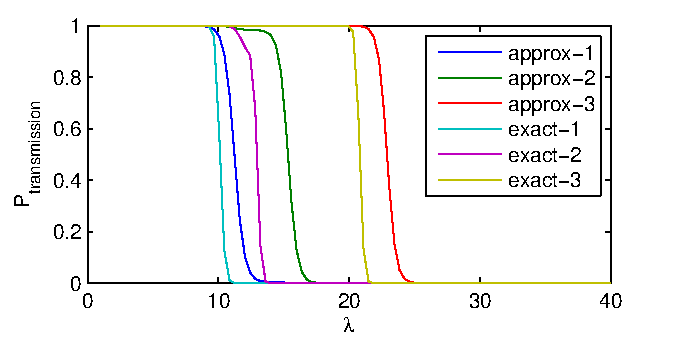
\includegraphics[width=\columnwidth]{results/plotPtransmission_exact_vs_approx.pdf}
  \caption{Comparing the approximate $\Ptrans$ with exact version. The drop in approximate version of $\Ptrans$ is delayed because we assume drop at the center of the car rather than camera facing face of the car.}
  \label{fig:compare:exact:approx:ptrans}
\end{figure}

Thus, we have modeled the transmission probability to effectively capture the effect of occlusion due to all traffic participants in a scene that lie along a particular ray. We reiterate that our reflection and transmission probabilities are continuous functions, which allows us to define continuous energy functions for association and 3D object localization, as described in the next section.

%\paragraph{Probabilistic occlusion levels}
%With the above modeling and using \eqref{eq:imgform}, 



%% We model the probability of a point $\mathbf{x}_j$ on a object $i$ getting successfully
%% observed in a camera image at point $\trackpj{t}$ is dependent up two factors,
%% (1) reflection and (2) transmission through intermediate space. The reflection
%% part ensures that there is an object to reflect a point at a certain region in
%% the 3D space while transmission part models occlusion.
%% \begin{align}
%%   P^{(ij)}_{\text{observation}} = P^{(ij)}_{\text{reflection}}P^{(j)}_{\text{transmission}}
%% \end{align}

%% %%%%%%%%%%%%%%%%%%%%%%%%%%%%%%%%%%%%%%%%%%%%%%%%%%%%
%% \subsection{Reflection probability}
%% For Lambertian reflection we replace the surface normal with the
%% gradient of occupancy.
%% %
%% \begin{align}
%%   \Prefl = (\max \{0, \nabla \occf^\top
%%   \hat{\mathbf{r}_j}\})^2
%% \end{align}
%% %
%% where $\ray =
%% \frac{K^{-1}\trackpj{t}}{\|K^{-1}\trackpj{t}\|}$ is unit vector in the
%% direction of ray. The gradient in the direction opposite to ray yields -ve
%% probability which needs to be clipped off. Squaring the function keep it
%% smooth near zero.

%% %%%%%%%%%%%%%%%%%%%%%%%%%%%%%%%%%%%%%%%%%%%%%%%%%%%%
%% \subsection{Transmission probability}
%% A model for transmission of light through a material of thickness $x$,
%% density $\rho$ and opacity $k_o$ is given by Beer-Lambert law 
%% %
%% \begin{align}
%%   I(x) = I_0e^{-k_o\rho x}
%% \end{align}
%% %

%% Since both opacity and density are represented by the occupancy function
%% $\occftot = \sum_i \occf$, and also the domain of our $\occftot$ is $[0, 1]$ instead of $[0,
%% \infty]$ as in case of $k_o$; we replace $e^{-k_o\rho}$ by the transparency
%% function $1 - \occftot$. So the transmission probability over a small distance
%% $d\lambda$ is given by
%% %
%% \begin{align}
%%   P_{\text{transmission}}(\lambda + d\lambda) =
%%   P_{\text{transmission}}(\lambda) (1-\occftot)^{d\lambda}
%% \end{align}
%% %

%% For a given 3D point $\mathbf{x}_j = \lambda \ray$, the probability that the
%% point $\trackpj{t}$ is reflected from a distance $\lambda$ is given by

%% \begin{align}
%%   %P^{(j)}_{\text{observation}}(\lambda) &= P_{\text{reflection}}
%%   \Ptrans &=
%%   \prod_{0}^{\lambda} (1 - \occft{\lambda \ray})^{d\lambda} %\\
%%   %= \max \{ 0, (\nabla f_{occ}&(\lambda \ray)^\top \ray) \}
%%   %\prod_{0}^{\lambda} (1 - f_{occ}(\lambda \ray))^{d\lambda}
%%   \label{eq:ptrans-integral}
%% \end{align}
%% where $\prod_{0}^{\lambda}$ represents the \emph{product integral} from $0$ to
%% $\lambda$. 

%% In practice, the integral for transmission probability
%% \eqref{eq:ptrans-integral} is difficult to compute even numerically. So we
%% choose a product of sigmoid function that approximates the behaviour of
%% transmission probability,
%% %
%% \begin{align}
%% \label{eq:evalCumulativePtrans}
%%   \Ptrans &= \prod_i L_u(\trackp{t}; \muiu,\Sigmaiu)L_{\lambda}(\lambda; \mu^i_d)
%% \end{align}
%% %
%% where $L_u(.)$ is sigmoid in image domain with $\mu^i_u$ and $\Sigma^i_u$
%% representing the elliptical projection of $i^{th}$ TP.
%% $L_{\lambda}(.)$ is sigmoid in the depth domain with $\mu^i_d$ as the mean
%% depth of the $i^{th}$ TP.
%% %
%% \begin{align}
%%   L_u(\mathbf{u}; \muiu,\Sigmaiu) &= \frac{1}{
%%     1 + e^{-k_u(1 - (\mathbf{u} - \muiu)^\top\Sigmaiu(\mathbf{u} -
%%     \muiu))}
%%   }
%%   \\
%%   L_{\lambda}(\lambda; \mu^i_d) &= \frac{1}{
%%     1 + e^{-k_d(\lambda - \mu^i_d)}
%% }
%% \end{align}
%% %

%% \begin{comment}%% Comment
%%   A product integral is a simple integral in log domain
%%   \begin{align}
%%     \prod_{0}^{\lambda} (1 - f_{occ}(\lambda \ray))^{d\lambda} =
%%     e^{\int_{1}^{\lambda} \ln{(1 - f_{occ}(\lambda \ray))}{d\lambda}}
%%   \end{align}
%% \end{comment}%% Comment

% \paragraph{Notation}
% We summarize the notation used in the report for quick reference.
% \\
% 
% 
%   \begin{tabular}{|l|l|}
%     \hline
%     Symbol & Meaning \\
%     \hline
%     $\pos{i}{t}$ & Position of $i$th car at time $t$\\
%     $\ori{i}{t}$ & Orientation of $i$th car at time $t$\\
%      $\dimsn{i}$ & 3D bounding box of the car (dimensions)\\
%     $\state{i}{t}$ & State of car $=\{\pos{i}{t}, \ori{i}{t}, \dimsn{i}\}$\\
%     $\egop$ & Position of camera at time $t$\\
%     $\egoo$ & Orientation of camera at time $t$\\
%     $\relp{i}{t}$ & Relative car pose w.r.t. camera \\
%     $\tracklets$ & 3D points tracked on car $i$ in its own frame\\
%     $\trackp{t}$ & Projection of $\tracklets$ in camera\\
%     $\projectionOf{.}$ & Projection function for pose $\relp{i}{t}$\\
%     $\bb{i}$ & 2D bounding box of the car in image\\
%     \hline
%   \end{tabular}

% 2.3 Point tracks
% 2.4 Object detections
With the understanding of our occlusion aware 3D representation of objects, we are know in position to describe the energies that we defined in Chapter~\ref{sec:setup}

%%%%%%%%%%%%%%%%%%%%%%%%%%%%%%%%%%%%%%%%%%%%%%%%%%%%
\section{Point tracks energy with occlusion}
\label{sec:totalContPtTracksEnergy}
We model continuous point tracks energy with explicit occlusion reasoning as
the expected re-projection error over the association probability,

\begin{align}
  \Energy{track}(\{ \relp{i}{t} \}_i, \{ \relp{i}{t-1} \}_i, \{\dimsn{i}\}_i ) = 
    \sum_{i=1}^{N} 
    %\sum_{t = s_i}^{e_i}
    \sum_{j = 1}^{M}
    \int_1^\infty \assocP\Ereproj(\lambda) d\lambda
\end{align}
where $\assocP$ is the association probability of
$j$\textsuperscript{th} point with $i$\textsuperscript{th} TP at depth $\lambda$, $\{ \relp{i}{t} \}_i$ are the poses of all occluding objects at time $t$, $ \{ \dimsn{i} \}_i$ are the dimensions of all objects that occlude $i$
and $\Ereproj(\lambda)$ is the re-projection error given by
%
\begin{align}
  \assocP &= \Prefl\Ptrans\\
  \Ereproj(\lambda) &= \left\|\trackpj{t} - \projectionOf{\invProjectionOftm{\trackpj{t-1}, \lambda}}\right\|^2 .
  \label{eq:reprojerror}
\end{align}

The  $\projectionOf{.}$ and $\invProjectionOftm{.}$ denote the projection and
inverse projection functions that project 3D point to camera image and vice
versa. Note that inverse projection $\invProjectionOf{.}$ depend on both the
point $\trackp{t}$ and the unknown depth $\lambda$. Also note that the inverse projection is dependent on TP pose at time $t-1$ while the projection depends on pose at time $t$ which can be different.

\begin{comment}
  \subsection{Occupancy function}
  Assuming occupancy to be a
  probability distribution over 3D space. For each TP the
  occupancy is modeled as a logistic function 
  \begin{align}
     \occf = L(\mathbf{x}; \pos{i}{t}, \Sigma_i)
  \end{align}
  where $L(.)$ is the logistic function defined by
  \begin{align}
    L(\mathbf{x}; \pos{i}{t-1}, \Sigma_i) = \frac{1}{
      1 + e^{-k(1 - d(\mathbf{x},\pos{i}{t-1}))}
      }
  \end{align}
  where $d(\mathbf{x},\pos{i}{t-1}) =
  (\mathbf{x}-\pos{i}{t-1})^\top\Sigma_i(\mathbf{x}-\pos{i}{t-1})$ and $k =
  10\ln{49}$. $k$ is chosen such that $L(.) = 0.98$ when $d(.) =
  0.9$
  % Once we have our distribution over $\lambda$, $\lambdadist$ we can compute the
  % reprojection of $\trackpj{t-1}$ over image in time $t$ as a function of
  % $\lambda$. Let
\end{comment}


\begin{comment}
  \subsection{Approximations}
  Reflection probability of $i$th TP is easy to compute
  analytically 
  \begin{multline}
    \Prefl =
    (\max \{ 0, \nabla \occf^\top \ray \})^2 \\
    = (\max \{ 0, \nabla \occfxi^\top\ray \})^2
    \label{eq:analytic-prefl}
  \end{multline}
  where 
  \begin{multline}
    \nabla \occfxi^\top\ray \\=
    \nabla k\dishort \sech^2\left(\frac{k}{2}\dishort\right)
  \end{multline}
  where $\dishort = 1-d(\mathbf{x}, \pos{i}{t-1})$ is a signed distance measure
  from the contour of the ellipsoid where $d(\mathbf{x}, \pos{i}{t-1})$ is 1.

  However, the transmission probability needs to be approximated.  
  %
  % \subsection{Computing $\Prefl$ and $\Ptrans$}
  % Focusing on  $\nabla \occfxi$ 
  % 
  % \begin{multline}
  %   \nabla \occfxi =\\
  %   \frac{-k\nabla d(\mathbf{x}, \pos{i}{t-1})e^{-k(1-d(\mathbf{x}, \pos{i}{t-1}))}}{
  %     (1 + e^{-k(1-d(\mathbf{x}, \pos{i}{t-1}))})^2
  %   } \\ 
  %   = -k\nabla d(\mathbf{x}, \pos{i}{t-1})\sech^2\left(\frac{k}{2}(1-d(\mathbf{x},
  %   \pos{i}{t-1}))\right)
  %   \\
  %   = \nabla k\dishort \sech^2\left(\frac{k}{2}\dishort\right)
  % \end{multline}
  % where $\dishort = 1-d(\mathbf{x}, \pos{i}{t-1})$ is a signed distance measure
  % from the contour of the ellipsoid where $d(\mathbf{x}, \pos{i}{t-1})$ is 1.
  % Focusing on $\nabla d(.)$
  % 
  % \begin{align}
  %   \nabla d(\mathbf{x}, \pos{i}{t-1}) = 2\Sigma_i(\mathbf{x} - \pos{i}{t-1})
  % \end{align}
  % Back to \eqref{eq:analytic-prefl}
  % 
  % \begin{multline}
  %   (\max \{ 0, \nabla \occf^\top \ray \})^2 = \\
  %   \sech^4\left(\frac{k}{2}\dishort\right) 
  %   (\max \{ 0 , \nabla k\dishort^\top\ray\})^2
  % \end{multline}
  % 
  % The probability is simply $\sech^2(.)$ scaled by gradient of ellipsoid
  % $\nabla k\dishort$ projected in the ray direction $\ray$.
  % 
  % \begin{align}
  %   \Ptrans = 
  %   e^{\int_{1}^{\lambda} \ln{(1 - f_{occ}(\lambda \ray))}{d\lambda}}
  % \end{align}
  % \begin{multline}
  % \int_{1}^{\lambda} \ln{(1 - f_{occ}(\lambda \ray))}{d\lambda}
  % =  \\
  % \int_{1}^{\lambda} \ln{\left(1 - \sum_i \occfi\right)}{d\lambda}
  % \end{multline}
  % 
  % The above integral is very difficult to approximate or compute analytically.
  So based on intuition, we approximate the $\Ptrans$ by following function
  \begin{align}
  \label{eq:evalCumulativePtrans}
    \Ptrans &= \prod_i L_u(\mathbf{u}, \mu^i_u,\Sigma^i_u)L_{\lambda}(\lambda; \mu^i_d)\\
    L_u(\mathbf{u}, \mu^i_u,\Sigma^i_u) &= \frac{1}{
      1 + e^{-k_u(1 - (\mathbf{u} - \mu^i_u)^\top\Sigma^i_u(\mathbf{u} -
      \mu^i_u))}
    }
    \\
    L_{\lambda}(\mathbf{u}, \lambda; \mu^i_d) &= \frac{1}{
    1 + e^{-k_d(\lambda - \mu^i_d(\mathbf{u}))}
  }
  \end{align}
  where 
  \begin{align}
    \mu_u^i &= \projectionOf{\pos{i}{t-1}} \label{eq:muiudef}\\
    \Sigma_u^i &= \projectionOf{\Sigma_i} \label{eq:sigmauidef}\\
    \mu^i_d(\mathbf{u}) &= \relp{i}{t}\\
    k_u &= 10\log(49)\\
    k_d &= \frac{\log(49)}{\sqrt{h^2 + l^2 + w^2}}
    \label{eq:ptransmissionInit}
  \end{align}
  is the distance of the centre of the TP from the camera.

  % $\mu^i_d(\mathbf{u}) = \min_{\lambda} d^2_i(\lambda K^{-1}\mathbf{u})$.
  % $\mu^i_d(\mathbf{u})$ is the closest point to the unit contour of ellipsoid.
  % If there are multiple such points, the point closest to the camera is taken as
  % $\mu^i_d(\mathbf{u})$

  The association probability becomes

  \begin{multline}
    \assocP = 
      \sech^4\left(\frac{k}{2}\dishort\right)
      (\max \{ 0, \nabla k\dishort^\top\ray \})^2\\
    \prod_i \Lu
      \Llambda \\
      \label{eq:assocCoeffEval}
  \end{multline}

  So the energy becomes

  \begin{multline}
    \label{eq:integrand}
    \Energy{track}(.) = 
      \sum_{i = 1}^N
      \sum_{j = 1}^{M}
      \int_1^{\infty}
      \assocP
      \Ereproj(\lambda)
      d\lambda
  \end{multline}
  where $x = \lambda \ray$ and $\Ereproj(\lambda) = \|\trackpj{t} -
  f^i_{reproj}(\trackpj{t-1}, \lambda)\|^2$ is reprojection error which is a
  quadratic in $\lambda$

  The integral in the above expression is computed numerically.
\end{comment}

\section{Object detection energy}

We model object detection energy as the norm of difference in the coordinates
of the projected bounding box and detected bounding box. The detected bounding
box is represented by the extrema along X and Y dimensions $\bb{i} = [\xmin,
\ymin, \xmax, \ymax]^\top$. If $\dimsn{i} = [l, w, h]^\top$ represent the 3D
dimensions of the traffic participant along the X, Y and Z dimensions then we 
can compute the eight corners of the cuboid model in the tracklet coordinate transform as

\begin{align}
  X^{(i)}_{\text{cuboid}} &= \dimsn{i}{}^\top C_u \\
  \text{where} &\\
  C_u &= 
  \begin{bmatrix}
  0.5 & 0.5 & -0.5 & -0.5 & 0.5 & 0.5 & -0.5 & -0.5 \\
    0.5 & -0.5 & -0.5 & 0.5 & 0.5 & -0.5 & -0.5 & 0.5 \\
    0 & 0 & 0 & 0 & 1  & 1 & 1 & 1
  \end{bmatrix} \enspace .
\end{align}
These cuboid points can be projected to the camera image plane to get the projected bounding box,
\newcommand{\ucub}{U^{(i)}(t)}
\newcommand{\ucubx}{U_{(1,:)}^{(i)}(t)}
\newcommand{\ucuby}{U_{(2,:)}^{(i)}(t)}
\newcommand{\estbb}{\hat{\mathbf{d}}^{(i)}(t)}
\begin{align}
  \ucub &= \projectionOf{\dimsn{i}{}^\top C_u}\\
  \estbb &= [\min \ucubx, \min \ucuby, \max \ucubx, \max \ucuby]^\top \enspace .
\end{align}
We take $\estbb$ as the projected bounding box. The object detection energy is
taken to be the euclidean distance between projected and detected bounding box.
\begin{align}
  \EnergyBBox &= \| \estbb - \bb{i}\|^2_2
\end{align}
With slight abuse of notation for projection operator we write this energy as
\begin{align}
  \EnergyBBox &= \left\| \projectionOf{\dimsn{i}} - \bb{i}\right\|^2_2 \enspace.
\end{align}

For object detections we use object detector by \cite{Felzenszwalb_etal_2010}
which is detector by parts model and we use eight parts to train the car model 
on half of the KITTI dataset \cite{geiger2013vision}. The trained modeled is 
used to get detections for the other half of the dataset and vice versa.

\section{Lane energy}
\label{sec:laneEnergy}
 The lanes are modeled as splines. Here we assume that the confidence in lane
 detection is decreases as the distance from the lane center increases.  The
 energy is given by the dot product between car orientation and tangent to the
 lane at that point.

\begin{align}
  \label{eq:laneOrientationEnergy}
  \Energy{lane} = 
  \sum_{m \in M_{\text{close}}}
  (1 - \ori{i}{t} \cdot \text{TAN}(L_{m}(k), \pos{i}{t}) )
\LaneUncertainty{\pos{i}{t}}
\end{align}
where $M_{\text{close}} = \{m : \text{DIST}(L_{m}(k), \pos{i}{t}) < d_{\text{thresh}}\} $ is
the set of nearby lanes close to the object by a certain distance threshold $d_{\text{thresh}}$ and 
\begin{align}
\LaneUncertainty{\pos{i}{t}} = 
  \frac{1}{1 + \exp(-q(w_{\text{road}} - \text{DIST}(L_{m}(k), \pos{i}{t})))}
\end{align}
for some constant $w_{\text{road}}$ that represents the width of the road.

\section{Transition probability}
Dynamics constraints should not only enforce smooth trajectories, but also the
holonomic constraints.  The following energy adds a penalty if the change in
position is not in direction of previous orientation.

\begin{align}
  \label{eq:totalPosTransitionEnergy}
  \Energy{dyn-hol} = 1 - \ori{i}{t-1} \cdot (\pos{i}{t} - \pos{i}{t-1})
\end{align}

The following energy adds a penalty for change in position and orientation
but a penalty for change in velocity is much better approximation. However, in
a Markovian setting that would mean extending the state space of the car to
include velocity.

\begin{align}
  \Energy{dyn-ori} &= \|\ori{i}{t} - \ori{i}{t-1}\|^2\\
  \Energy{dyn-vel} &= \|(\pos{i}{t} - 2\pos{i}{t-1}) + \pos{i}{t-2}\|^2
\end{align}

As a result the dynamics are modeled by weighted combination of holonomic
constraint and smoothness constraints.

\begin{align}
  \WEnergy{dyn} &= \WEnergy{dyn-hol} + \WEnergy{dyn-ori} + \WEnergy{dyn-vel}
\end{align}

 
\section{Collision energy}

Bhattacharya coefficient $\int_a^b\sqrt{p(x)q(x)}dx$ is a measure of similarity
of two distributions $p(x)$ and $q(x)$. If we represent TPs as gaussians in
Birds eye view (BEV), then similarity is a measure of collision. Exactly
overlapping distribution results in coefficient as 1. 
%The analytical form of
%Bhattacharya coefficient has been taken from
%\url{http://like.silk.to/studymemo/PropertiesOfMultivariateGaussianFunction.pdf}

\begin{align}
  \label{eq:collisionEnergyHellingerDistance}
  \EnergyCol =
  -\log\left(
  A_{ij}
  e^{-\frac{1}{8}
    \left(\pos{i}{t} - \pos{j}{t}\right)^\top
    P^{-1}
    \left(\pos{i}{t} - \pos{j}{t}\right)
    }
    \right)
\end{align}
where 
\begin{multline}
  A_{ij} = \frac{|\Sigma_i|^\frac{1}{4}|\Sigma_j|^\frac{1}{4}}{|P|^\frac{1}{2}}, \hfill
  P = \frac{1}{2}\Sigma_i + \frac{1}{2}\Sigma_j, \hfill
\Sigma_i^{-1} = R^\top_{\ori{i}{t}} \begin{bmatrix} 2/l_i & 0 \\ 0 & 2/w_i \end{bmatrix}
R_{\ori{i}{t}}
\end{multline}


\section{Size Prior}

Prior can include among many other things the size prior on the car.

\begin{align}
  \label{eq:totalSizeEnergy}
  \Energy{size} &= (\dimsn{i} - \expDimsn)^\top\Sigma_{\expDimsn}^{-1}(\dimsn{i} -
  \expDimsn)
\end{align}

where $\expDimsn$ is the mean TP dimensions and
$\Sigma_{\expDimsn}$ is the correspondence covariance matrix.


%
% 3. Inference
% 3.1 fminunc
% 3.2 Particle belief propagation
% 3.3 MCMC
%We use two methods for inference, Metropolic Hastings and block coordinate descent. We briefly describe the inference algorithms for completeness.

\section{Metropolis Hastings}
Metropolis Hastings requires a \emph{transition probability} $Q(\map'|
\map^r)$, that depends on current sample $\map^r$ and guides
the random walk in the high-dimensional space. We randomly sample a point
$\map'$ from from $Q(.)$ and it is either accepted or rejected based on the
\emph{acceptance probability} $a$:
\begin{align}
  a = \frac{P(\map')Q(\map^r| \map')}
  {P(\map^r)Q(\map'| \map^r)}
  \enspace,
\end{align}
where $P(\map)$ is joint probability of the model at point $\map$.

If $a \ge 1$, then the new point $\map'$ is accepted otherwise it is accepted
with probability $a$. Here acceptance means that the point in the next
iteration is taken as the sampled point otherwise the earlier point is retained.

\section{Block Coordinate Descent}

We use block coordinate descent algorithm on our factor graph, by iteratively
minimizing the energy with respect to only a subset (block) of random 
variables. We choose to divide the blocks along the
variable types like dimension, yaw and position. Hence we iteratively minimize the energies with respect to dimension variables, then with respect to yaw variables and then with respect to position variables. Since we know the dependence of parts of our energy on specific variables, thanks to factor graph formulation, we can minimize the energies corresponding to the given set of variables.


%
% 4. Experments and Results
% 4.1 Prove that PGM is useful
% 4.2 Prove that Adding GPS/Lane information is useful
% 4.3 Prove that Adding Point tracks energy is useful
% 4.4 Prove that Adding Occlusion model is useful/not useful
\section{Experiments}
\label{sec:experiments}

In this section, we first compare our continuous occlusion model for point-to-object association against the baseline method using detection bounding boxes and state-of-the-art methods for motion segmentation. We then show how the proposed model benefits the task of 3D localization in autonomous driving.

For our experiments, we use the KITTI dataset~\cite{geiger2013vision}, which consists of video sequences of road scenes under a variety of driving conditions including highways and residential areas. It also provides ground truth data for different tasks such as segmentation, detection, tracking and 3D localization.

%\paragraph{Dataset} We use KITTI dataset for our experiments.  \cite{geiger2013vision}. KITTI dataset is a labeled video sequence of road scenes under variety of driving conditions including highways and residential areas in Karlsruhe, Germany. It provides manually labelled ground truth data for localization of cars and also uses velodyne data provide metrically accurate estimates of cars location.


%%%%%%%%%%%%%%%%%%%%%%%%%%%%%%%%%%%%%%%%%%%%%%%%%%%%
\subsection{Association experiment}

We first perform the association experiment that compares the accuracy of point-to-object association using the proposed model against those of detection bounding box baseline method (BBox) and state-of-the-art motion segmentation methods, namely robust algebraic segmentation with hybrid perspective constraints (RAS)~\cite{Rao_etal_2010} and spectral clustering with point track spatial affinity (BM)~\cite{Brox_Malik_2010}.

%To verify the correctness of our association probability $\assocP$ we perform association error experiment that compare the accuracy of point track association with TPs with that of bounding box baseline method.

\subsubsection{Association probability}

Using our continuous occlusion model in Section~\ref{sec:setup}, the association probability $\assocP$ of $j$\textsuperscript{th} point track with $i$\textsuperscript{th} object at depth $\lambda$ can be defined as
\begin{align}
  \assocP = \Prefl\Ptrans,
\end{align}
where $\Prefl$ and $\Ptrans$ are from \ref{eq:evalPrefl} and \ref{eq:evalCumulativePtrans} respectively. Note that the fraction $\assocP$ although called association probability does not capture the entire information that we have available for computing association of point tracks to objects. This above fraction is the association probability given the hypothesized parameters of TPs. 

To compute the association probability $\assocP$ between point track $j$ and TP $i$ we must use re-projection error as well. When the association of $i$ and $j$ is correct and the point of reflection is at depth $\lambda$, the re-projection error must be zero \eqref{eq:reprojerror}, otherwise the error becomes a measure of distance from the true solution. The error terms can be converted to probability domain by considering the error term as negative log of probability
\begin{align}
  P^{(ij)}_{\text{assoc by reproj}}(\lambda) = \frac{1}{Z}\exp(-\Ereproj(\lambda))
\end{align}

Using both of the above evidence terms we can write the probability of association $P^{(ij)}_{\text{assoc}}$ as follows
\begin{align}
  P^{(ij)}_{\text{assoc}} = \frac{1}{Z'}\int_0^{\infty} \assocP \exp(-\Ereproj(\lambda))d\lambda
  \label{eq:prob-assoc}
\end{align}

Once we have the probability of association $P^{(ij)}_{\text{assoc}}$ we can compute the best possible assignment of TP for each point track. The points having very small association probability are assigned to the background,
\begin{align}
  i^*_{j} = \argmin_{i} \int_0^\infty \assocP \Ereproj(\lambda) d\lambda
\end{align}

We use detection bounding box based assignment of point tracks to TPs as the baseline. For the regions where the bounding boxes overlap, we assign the point tracks to the TP that has smaller mean depth than the competing bounding box.

\subsubsection{Association results}

For each sequence of the KITTI dataset, the methods of \cite{} and \cite{} are used respectively for computing detection bounding boxes and object tracklets. We then apply \cite{} on object tracklets to extract point tracks. From these point tracks, we create four different sets of input point tracks, namely all point tracks, occluded point tracks, dynamic point tracks and dynamic and occluded point tracks, to examine various aspects of the methods (our method focuses on occlusion scenes while RAS and BM favour dynamic scenes). In addition to point tracks, the parameters of all TPs estimated by the method~\cite{Song_Chandraker_2014} are provided to our method (for computing association probability) and the baseline method (for depth ordering).

Figure~\ref{fig:assoc-occ-results} presents the association errors --- the percentages of point tracks incorrectly assigned to objects --- of all methods on four sets of input point tracks for each sequence as well as the mean results over all sequences of the KITTI dataset. From the results, our method is usually the most accurate among all methods, leading to the best mean errors on all sets of input point tracks, which is followed by the bounding box baseline method. This clearly shows the advantage of our continuous occlusion model over the simple baseline method for resolving occlusions. Both RAS and BM often have the highest errors and hence the highest mean errors on all sets of input point tracks.

\begin{figure*}
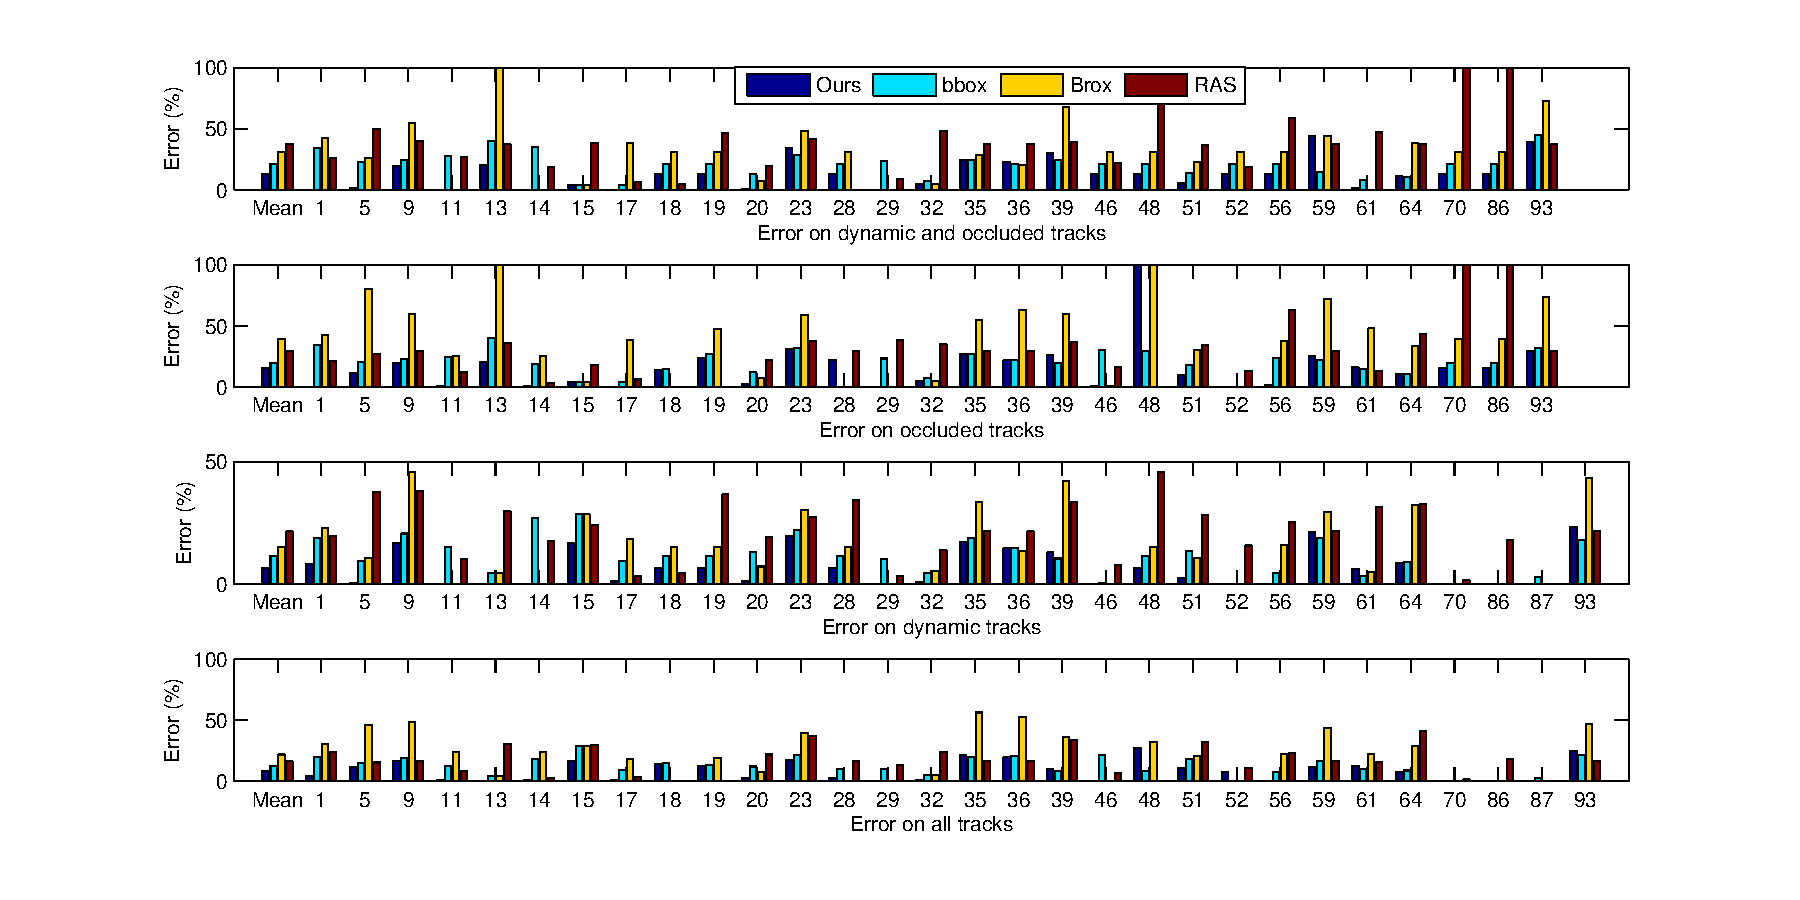
\includegraphics[trim=1.0in 0.4in 1.0in 0.2in, clip, width=\textwidth]{results/plotErrorBarEvalAssocCoeffAllSequence.pdf}
  \caption{Association errors on different sets of point tracks. The
    numbers on y-axis represent the data sequence number in KITTI dataset. The
    first set of bars in each plot correspond to the mean across all sequences.
    The error is in terms of average fraction of foreground points incorrectly
    associated to objects per sequence.}
\label{fig:assoc-occ-results}
\end{figure*}


\newlength{\tblimgwidth}
\setlength{\tblimgwidth}{0.40\textwidth}
\begin{table*}
  \centering
  \begin{tabular}{ccc}
    & Associations & Error in association\\
    \rotatebox{90}{\hspace{2em} Baseline} & 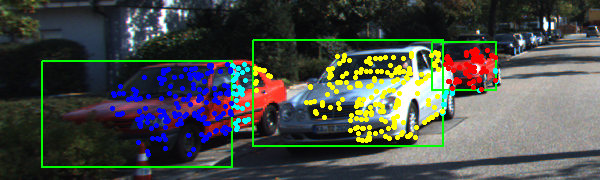
\includegraphics[width=\tblimgwidth]{results/0009_0000000060_point_assign_bbox2D_model-small.png} &%
    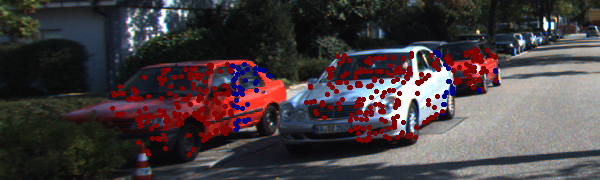
\includegraphics[width=\tblimgwidth]{results/0009_0000000060_point_assign_bbox2D_model_correct_incorrect-small.png}\\
    \rotatebox{90}{\hspace{2em} BM} & 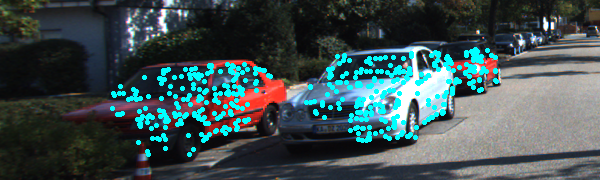
\includegraphics[width=\tblimgwidth]{results/0009_0000000060_point_assign_BroxAndMalik2010-small.png} &%
    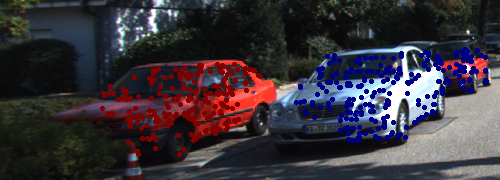
\includegraphics[width=\tblimgwidth]{results/0009_0000000060_point_assign_BroxAndMalik2010_correct_incorrect-small.png}\\
    \rotatebox{90}{\hspace{2em} RAS} & 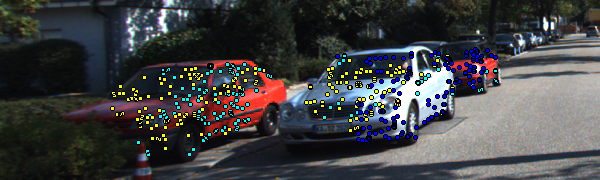
\includegraphics[width=\tblimgwidth]{results/0009_0000000060_point_assign_RAS-small.png} &%
    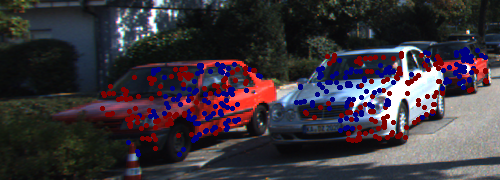
\includegraphics[width=\tblimgwidth]{results/0009_0000000060_point_assign_RAS_correct_incorrect-small.png}\\
    \rotatebox{90}{\hspace{2em} Ours} & 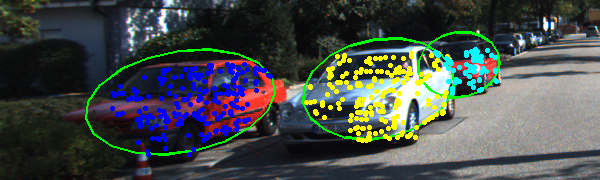
\includegraphics[width=\tblimgwidth]{results/0009_0000000060_point_assign_contPtTracks-small.png} &%
    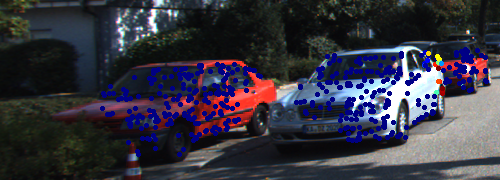
\includegraphics[width=\tblimgwidth]{results/0009_0000000060_point_assign_contPtTracks_correct_incorrect-small.png}\\
    \rotatebox{90}{\hspace{2em} Baseline} & 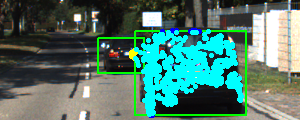
\includegraphics[width=\tblimgwidth]{results/0013_0000000060_point_assign_bbox2D_model-small.png} &%
    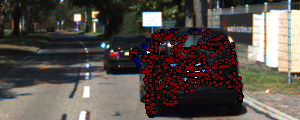
\includegraphics[width=\tblimgwidth]{results/0013_0000000060_point_assign_bbox2D_model_correct_incorrect-small.png}\\
    \rotatebox{90}{\hspace{2em} BM} & 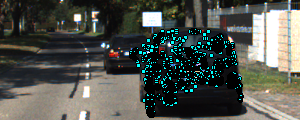
\includegraphics[width=\tblimgwidth]{results/0013_0000000060_point_assign_BroxAndMalik2010-small.png} &%
    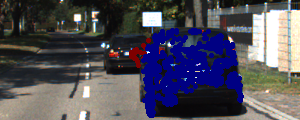
\includegraphics[width=\tblimgwidth]{results/0013_0000000060_point_assign_BroxAndMalik2010_correct_incorrect-small.png}\\
    \rotatebox{90}{\hspace{2em} RAS} & 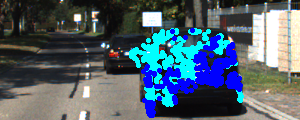
\includegraphics[width=\tblimgwidth]{results/0013_0000000060_point_assign_RAS-small.png} &%
    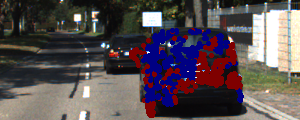
\includegraphics[width=\tblimgwidth]{results/0013_0000000060_point_assign_RAS_correct_incorrect-small.png}\\
    \rotatebox{90}{\hspace{2em} Ours} & 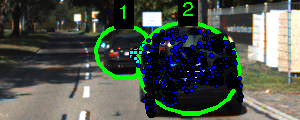
\includegraphics[width=\tblimgwidth]{results/0013_0000000060_point_assign_contPtTracks-small.png} &%
    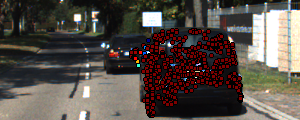
\includegraphics[width=\tblimgwidth]{results/0013_0000000060_point_assign_contPtTracks_correct_incorrect-small.png}
  \end{tabular}
  \caption{Qualitative results for association experiment. The left column
  shows the point tracks assignment to appropriate object. Each color represents
a different track to which the point is associated to. Right column shows the
probablistic error in association: red is low error while blue is high error.
Note that our method changes smoothly at the boundary of the objects with
intermediate probabilities, while the baseline methods have only 0-1 error.} 
\end{table*}

\subsection{Localization Experiment}
To show the effectiveness of our method we apply it to the localization
problem. We estimate the position, orientation and dimensions of the car with
our framework and compute the error in birds eye view domain along the ground
plane. We report error in three metrics translation error (t) in meters per
car, yaw error (yaw) in radians per car and dimension error is again meters per
car. The results are shown in Table~\ref{tab:localizationExperiment}.

We build the graphical model as shown in Fig~\ref{fig:graphmodel} that 
allows us to factorize the intractable probability distribution into following form
%
\begin{multline}
  -\log{P(\{\state{i}{t}\} | \mathbb{E})} = 
  -Z' 
  \\
  + \sum_{t=s_i}^{e_i}
  \left(
  \sum_{i,j:i\ne j}   
  \WEnergyCol 
   + \WpEnergy{bbox}
   + \WpEnergy{track}
\right)
  \\
  + \left(
  \sum_{i=1}^N 
  \WEnergy{lane}
  + \WEnergy{dyn}
  + \WEnergy{size}
\right)
  \enspace.
\end{multline}
%
We use the following energies in our graphical model.

\subsubsection{Continuous point tracks energy with occlusion}
\label{sec:totalContPtTracksEnergy}
We model continuous point tracks energy with explicit occlusion reasoning as
the expected re-projection error over the association probability,

\begin{multline}
  \Energy{track}(\{ \relp{i}{t} \}_i, \{ \relp{i}{t-1} \}_i, \{\dimsn{i}\}_i ) = 
  \\
    \sum_{i=1}^{N} 
    %\sum_{t = s_i}^{e_i}
    \sum_{j = 1}^{M}
    \int_1^\infty \assocP\Ereproj(\lambda) d\lambda
\end{multline}
where $\assocP$ is the association probability of
$j$\textsuperscript{th} point with $i$\textsuperscript{th} TP at depth $\lambda$, $\{ \relp{i}{t} \}_i$ are the poses of all occluding objects at time $t$, $ \{ \dimsn{i} \}_i$ are the dimensions of all objects that occlude $i$
and $\Ereproj(\lambda)$ is the re-projection error given by
%
\begin{align}
  \assocP &= \Prefl\Ptrans\\
  \Ereproj(\lambda) &= \left\|\trackpj{t} - \projectionOf{\invProjectionOftm{\trackpj{t-1}, \lambda}}\right\|^2 .
  \label{eq:reprojerror}
\end{align}

The  $\projectionOf{.}$ and $\invProjectionOftm{.}$ denote the projection and
inverse projection functions that project 3D point to camera image and vice
versa. Note that inverse projection $\invProjectionOf{.}$ depend on both the
point $\trackp{t}$ and the unknown depth $\lambda$. Also note that the inverse projection is dependent on TP pose at time $t-1$ while the projection depends on pose at time $t$ which can be different.

\subsubsection{Continuous bounding box energy with occlusion}

Object detection is usually followed by non-maximal suppression that results in
discarding similar bounding boxes. When we are jointly optimizing detections
with other cues, it is not usually desirable to go with a single bounding box.
Hence, we keep all the bounding box detections by approximating them with
multi-modal sum of Gaussian like logistic functions. We fit the parametric function of the form 
%
\begin{multline}
  S(\bb{i}) = \\
  \sum_k A_k \exp(-(\bb{i}-\mu^{(d)}_k)^\top \Sigma^{(d)-1}_k
  (\bb{i}-\mu^{(d)}_k))
\end{multline}
%
to detection scores, by non-linear error minimization with initialization from
non-maximal suppressed outputs. Here $\mu^{(d)}_j$ is one of the $k$ modes as a
4D vector representing a single bounding box as $[\minx, \miny, \maxx,
\maxy]^\top$. The optimization is constrained with symmetry and positive
definiteness of $\Sigma^{(d)-1}_k$, $\maxx \ge \minx$ and $\maxy \ge \miny$.

\paragraph{Detection scores with occlusion reasoning} 
\def\u{\mathbf{u}}
With our model of $\Ptrans$ described in Section \ref{sec:ptransmission}, we can
compute the probability of a point $\u$ on image be occluded assuming
the point is on traffic participant (TP) $i$ with mean depth $\mu^{(i)}_d$ as
\begin{align}
  O_{i}(\u, \mu^{(i)}_d) = 1 - \Ptransmission(\mu^{(i)}_d\u) \enspace .
\end{align}

If we know a portion of our proposed detection bounding box is known to be
occluded, then we would like to decrease the confidence in the detection score
about the localization of that end of the object. Assuming that the occlusion
is often on the boundary of detection bounding boxes, we want to decrease our
confidence on the mean detection boundaries around the occluded boundaries.
To re-model our detection scores scaled by continuous occlusion we sample
$O_{i}(\mathbf{u}, \mu^{(i)}_d)$ at the hypothesized detection boundaries from
GMM $S(.)$ and we augment the detection boundary covariance matrix by
$\mathcal{P}_{j} = \rho_{j}\rho_{j}^\top$ where $\rho_{j} = O_{j}(\mathbf{u},
\mu^{(i)}_d)$. The new covariance matrix in detection score is given by 
  $\Sigma'^{(d)}_j = \mathcal{P}_{j} + \Sigma^{(d)}_j$.
The detection scores GMM with occlusion is given by replacing the covariance
matrix
%
\begin{multline}
  S'(\bb{i}) =
  \\
  \sum_j A_j \exp(-(\bb{i}-\mu^{(d)}_j)^\top \Sigma'^{(d)-1}_j
  (\bb{i}-\mu^{(d)}_j))
\end{multline}

The energy of detection scores is simply take to be the inverse of the detection score.
\begin{align}
  \Energy{detect}(\{ \relp{i}{t} \}_i, \{ \relp{i}{t-1} \}_i, \{\dimsn{i}\}_i ) = \frac{1}{S'(\bb{i})}
\end{align}

For object detections we use object detector by \cite{Felzenszwalb_etal_2010}
which is detector by parts model and we use eight parts to train the car model 
on half of the KITTI dataset \cite{geiger2013vision}. The trained modeled is 
used to get detections for the other half of the dataset and vice versa. 

\subsubsection{Other energies}
Other energies we use are described in detail in the supplementary material. We briefly describe them here:
\begin{description}
  \item[Lane energy ($\Energy{lane}$)] This energy term constrains the
    orientation of traffic participants to be parallel to the nearest detected
    lane. The lanes are either detected visually or obtained from GPS and Map 
    information.
  \item[Transition probability ($\Energy{dyn}$)] We use these energies to
    constrain the motion of cars to be smooth in linear motion and rotation
    motion. We also constrain cars to move in the direction of heading.
  \item[Size prior ($\EnergySize$)] We use size prior of cars by using the mean
    of cars over the KITTI dataset.
\end{description}



\begin{figure}
  \centering
  \newcommand{\imagewidth}{\columnwidth}
  ../../CVPR/Source/scenelayoutoverlayCity0961.tex
  \caption{A sample road scene with the unknowns of each car modeled as random variables. 
  The relating energies are shown in Figure~\ref{fig:graphmodel}}
\end{figure}
\begin{figure}
    \usetikzlibrary{trees,shadows}
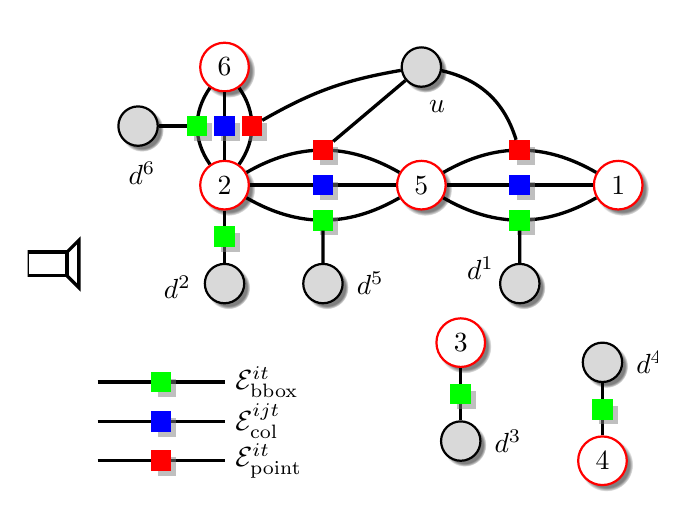
\begin{tikzpicture}[grow cyclic, line width=1.2pt,
    variablenode/.style={circle,circular drop shadow,draw=red,fill=white,thick,minimum width=0.5cm},
   bboxfactor/.style={rectangle,drop shadow,draw=green,fill=green,thick,minimum width=0.2cm},
    collfactor/.style={rectangle,drop shadow,draw=blue,fill=blue,thick,minimum width=0.2cm},
    trackfactor/.style={rectangle,drop shadow,draw=red,fill=red,thick,minimum width=0.2cm},
  obs/.style={fill=gray!30,draw=black},
  prevf/.style={draw=green!20,text=gray},
  prevobsv/.style={draw=gray!10,fill=gray!1,text=gray},
  prevv/.style={draw=red!20,text=gray}
]
  \path[use as bounding box,clip] (-2.5, -5.5) rectangle (5.5,0.5);
  \draw (-2.5,-2.65) rectangle +(0.5,0.3);
  \draw (-2.0,-2.35) -- ++(0.15, 0.15) -- ++(0, -0.6) -- (-2.0, -2.65);
\path
     (0, 0)  node [variablenode] (x6) {6}
++(0, -1.5) node [variablenode] (x2) {2}
++(2.5, 0)  node [variablenode] (x5) {5}
+ (0, 1.5)  node [variablenode,obs] (u) {}
+(.2,1.0)  node {$u$}
+ (.5, -2)   node [variablenode] (x3) {3}
+ (2.3, -3.5)   node [variablenode] (x4) {4}
+(2.5, 0)  node [variablenode] (x1) {1}
;

% Factors between nodes 6 and 2
\draw (x6) edge [bend right=35] node [bboxfactor] (f26) {} (x2);
\path (f26) +(-0.75,0) node [variablenode,obs] (d6) {} 
                        +(-.7,-.6)  node {$d^6$};
\draw (f26) edge (d6);
\draw (x6) edge [bend left=35] node [trackfactor] (ft26) {} (x2);
\draw (ft26) edge [bend left=10] (u);
\draw (x6) edge node [collfactor] {} (x2);

% Factors for node 2
\path (x2) +(0,-1.25) node [variablenode,obs] (d2) {} 
                        +(-.6,-1.3)  node {$d^2$};
\draw (x2) edge node [bboxfactor] {} (d2);

% Factors between nodes 2 and 5
\draw (x2) edge [bend right] node [bboxfactor] (f25) {} (x5);
\draw (x2) edge [bend left] node [trackfactor] (ft25) {} (x5);
\draw (x2) edge [] node [collfactor] {} (x5);
\draw (ft25) edge (u);
\path (x5) ++(-1.25,-1.25) node [variablenode,obs] (d5) {} 
                        +(.6,0)  node {$d^5$};
\draw (f25) edge (d5);

% Factors between nodes 5 and 1
\draw (x5) edge [bend right] node [bboxfactor] (f51) {} (x1);
\draw (x5) edge [bend left] node [trackfactor] (ft51) {} (x1);
\draw (x5) edge [] node [collfactor] {} (x1);
\draw (ft51) edge [bend right] (u);
\path (x1) ++(-1.25,-1.25) node [variablenode,obs] (d1) {} 
                        +(-.5,0.2)  node {$d^1$};
\draw (f51) edge (d1);

% Factors for node 3
\path (x3) ++(0,-1.25) node [variablenode,obs] (d3) {} 
                        +(.6,0)  node {$d^3$};
\draw (x3) edge node [bboxfactor] {} (d3);

% Factors for node 4
\path (x4) ++(0,1.25) node [variablenode,obs] (d4) {} 
                        +(.6,0)  node {$d^4$};
\draw (x4) edge node [bboxfactor] {} (d4);

% Legend
\path (-1.75,-4.0) node (l1s) {} (-0, -4.0) node [anchor=west] (l1e) {$\Energy{bbox}$};
\draw (l1s) edge node [bboxfactor] {} (l1e);
\path (-1.75,-4.5) node (l2s) {} (0, -4.5) node [anchor=west] (l2e) {$\EnergyCol$};
\draw (l2s) edge node [collfactor] {} (l2e);
\path (-1.75,-5.0) node (l3s) {} (0, -5.0) node [anchor=west] (l3e) {$\Energy{point}$};
\draw (l3s) edge node [trackfactor] {} (l3e);

\end{tikzpicture}

    \caption{Graphical model for a single frame with state of car represented
    as single node.  The six numbered nodes represent the unknown state variables of each car. The shaded nodes in the graphical model are observed variables. }
  \label{fig:graphmodel}
\end{figure}

\begin{table}
  \centering
  \begin{tabular}{lrrr}
    \toprule
    Energy & t & yaw & dim \\
    \midrule
    initialization                                                                                  & 3.79 & \textbf{0.86} & 1.64 \\
    $\EnergyLane+\EnergySize+\EnergyBBox+\EnergyDyn                                       $ & 3.83 & 0.90 & \textbf{1.14} \\
    %$\EnergyLane+\EnergySize+\EnergyBBoxocc+\EnergyDyn                                    $ & 3.83 & 0.90 & 1.14 \\
    %$\EnergyLane+\EnergySize+\EnergyBBoxocc+\EnergyDyn+\EnergyCol                         $ & 3.92 & 0.91 & 1.15 \\
    %$\EnergyLane+\EnergyContpttracks+\EnergySize+\EnergyBBoxocc+\EnergyDyn             $ & 3.81 & 0.92 & 1.59 \\
    % \EnergyBBox+\EnergyDyn+\EnergyCol $
    $\EnergyTrackNoOcc+\EnergyCol + \EnergyLane + \dots$  & 3.80 & 0.91 & 1.58 \\
    $\EnergyTrack+\EnergyCol + \EnergyLane + \dots$ & \textbf{3.78} & 0.91 & 1.58 \\
    \bottomrule
  \end{tabular}
  \caption{Localization experiment results with different combination of energies. We report error in three metrics translation error (t) in meters per car, yaw error (yaw) in radians per car and dimension error is again meters per car.}
  \label{tab:localizationExperiment}
\end{table}

% 
% 5. Conclusion and Discussions
\section{Discussion and Future Work}
\label{sec:discussions}

Our experiments shows that our association probability produces more accurate point to object associations when compared to simple bounding box based association. This shows that our occlusion aware 3D representation of objects works. However the localization experiment results do not show significant improvements by using more complicated models. 

% \section{Possible sources of error}
Since the results are averaged over the entire KITTI dataset, there are various possible sources of error, including outliers in point tracks, outliers in detections results. By noting that the dimension error is lower for fewer energies and translation error follows a relatively unpredictable trend, we stress on the requirement of learning of energy weights $\lambda_{\text{col,bbox,track,lane,dyn,size}}$. However, because of slow inference algorithms, which take about a day to run on 300 cores for the entire KITTI dataset, learning become infeasible.

%\section{Possible ways of improving the results}
We have several ideas for speeding up inference and thereby allowing learning
of weights to become feasible. One of them is to approximate the graph into a tree using Chow-Liu's \cite{chow1968approximating} algorithm and then using Belief Propagation which is linear in the number of edges of the tree.


{\small
  \bibliographystyle{ieee}
  \bibliography{continuousocclusion}
}
\end{document}

  
